\documentclass[11pt,border=4pt]{standalone}
% Estilo comum dos fluxogramas do Caderno C3 (cores do modelo do MOP)
\usepackage[T1]{fontenc}
\usepackage[utf8]{inputenc}
\usepackage{helvet}
\renewcommand{\familydefault}{\sfdefault}
\usepackage{amssymb}
\usepackage{tikz}
\usetikzlibrary{positioning, arrows.meta, shapes.geometric, shapes.symbols, shapes.misc,
  calc, fit, backgrounds, decorations.pathmorphing, patterns, shadows}
% Paleta do modelo do caderno
\definecolor{cTeal}{HTML}{00747A}
\definecolor{cNavy}{HTML}{0B3A5A}
\definecolor{cBlue}{HTML}{0A73BA}
\definecolor{cBlueBg}{HTML}{EBF4F9}
\definecolor{cTealBg}{HTML}{E3F1F2}
\definecolor{cTealMid}{HTML}{9CCFD2}
\definecolor{cGrayBg}{HTML}{F2F2F2}
\definecolor{cGrayLine}{HTML}{BFBFBF}
\definecolor{cGrayText}{HTML}{595959}
\definecolor{cText}{HTML}{1A1A1A}
\definecolor{cAmber}{HTML}{B7791F}
\definecolor{cAmberBg}{HTML}{FDF3DC}
\definecolor{cGreen}{HTML}{3D7D3A}
\definecolor{cGreenBg}{HTML}{E8F2E4}
\color{cText}
\tikzset{
  every node/.style={font=\footnotesize, text=cText},
  etapa/.style={draw=cTeal, fill=cTealBg, rounded corners=2pt, align=center,
     inner sep=3.5pt, minimum height=0.85cm, text width=#1, line width=0.6pt},
  etapa/.default={3.2cm},
  marco/.style={draw=cNavy, fill=cNavy, rounded corners=2pt, align=center,
     inner sep=3.5pt, minimum height=0.85cm, text width=#1,
     font=\footnotesize\bfseries, text=white},
  marco/.default={3.2cm},
  marcoteal/.style={draw=cTeal, fill=cTeal, rounded corners=2pt, align=center,
     inner sep=3.5pt, minimum height=0.85cm, text width=#1,
     font=\footnotesize\bfseries, text=white},
  marcoteal/.default={3.2cm},
  externo/.style={draw=cGrayLine, fill=cGrayBg, rounded corners=2pt, align=center,
     inner sep=3.5pt, minimum height=0.85cm, text width=#1},
  externo/.default={3.2cm},
  produto/.style={draw=cTeal!70, fill=white, rounded corners=1pt, align=center,
     inner sep=2.5pt, minimum height=0.6cm, text width=#1, font=\scriptsize},
  produto/.default={2.4cm},
  decisao/.style={draw=cAmber, fill=cAmberBg, diamond, aspect=2, align=center,
     inner sep=1pt, font=\scriptsize, line width=0.6pt},
  correcao/.style={draw=cAmber, fill=cAmberBg, rounded corners=2pt, align=center,
     inner sep=3pt, minimum height=0.8cm, text width=#1, font=\scriptsize},
  correcao/.default={2.6cm},
  transversal/.style={draw=cBlue, fill=cBlueBg, dashed, rounded corners=2pt, align=center,
     inner sep=3.5pt, text width=#1, line width=0.6pt},
  transversal/.default={6cm},
  seta/.style={-{Stealth[length=2.2mm,width=1.8mm]}, line width=0.8pt, draw=cNavy},
  setaleve/.style={-{Stealth[length=1.8mm,width=1.5mm]}, line width=0.6pt, draw=cGrayText},
  setatracejada/.style={-{Stealth[length=2mm]}, line width=0.7pt, dashed, draw=cGrayText},
  rotulo/.style={font=\scriptsize\itshape, text=cGrayText, fill=white, inner sep=1pt},
  fase/.style={signal, signal to=east, signal from=west, draw=cTeal, fill=cTealBg,
     align=center, font=\scriptsize\bfseries, minimum height=1.05cm, text width=#1,
     inner sep=2pt},
  fase/.default={1.9cm},
  raia/.style={draw=cGrayLine, fill=cGrayBg, minimum width=#1, minimum height=0.9cm,
     anchor=north west},
  tituloraia/.style={font=\scriptsize\bfseries, text=cNavy, align=center, text width=1.75cm},
  cab/.style={font=\scriptsize\bfseries, text=white, fill=cNavy, align=center,
     inner sep=3pt, text width=#1, minimum height=0.6cm},
  cab/.default={3cm},
  bloco/.style={draw=cGrayLine, fill=cGrayBg, rounded corners=3pt},
}
% sem hifenização nas caixas dos fluxogramas
\AtBeginDocument{\hyphenpenalty=10000 \exhyphenpenalty=10000 \sloppy}

\begin{document}

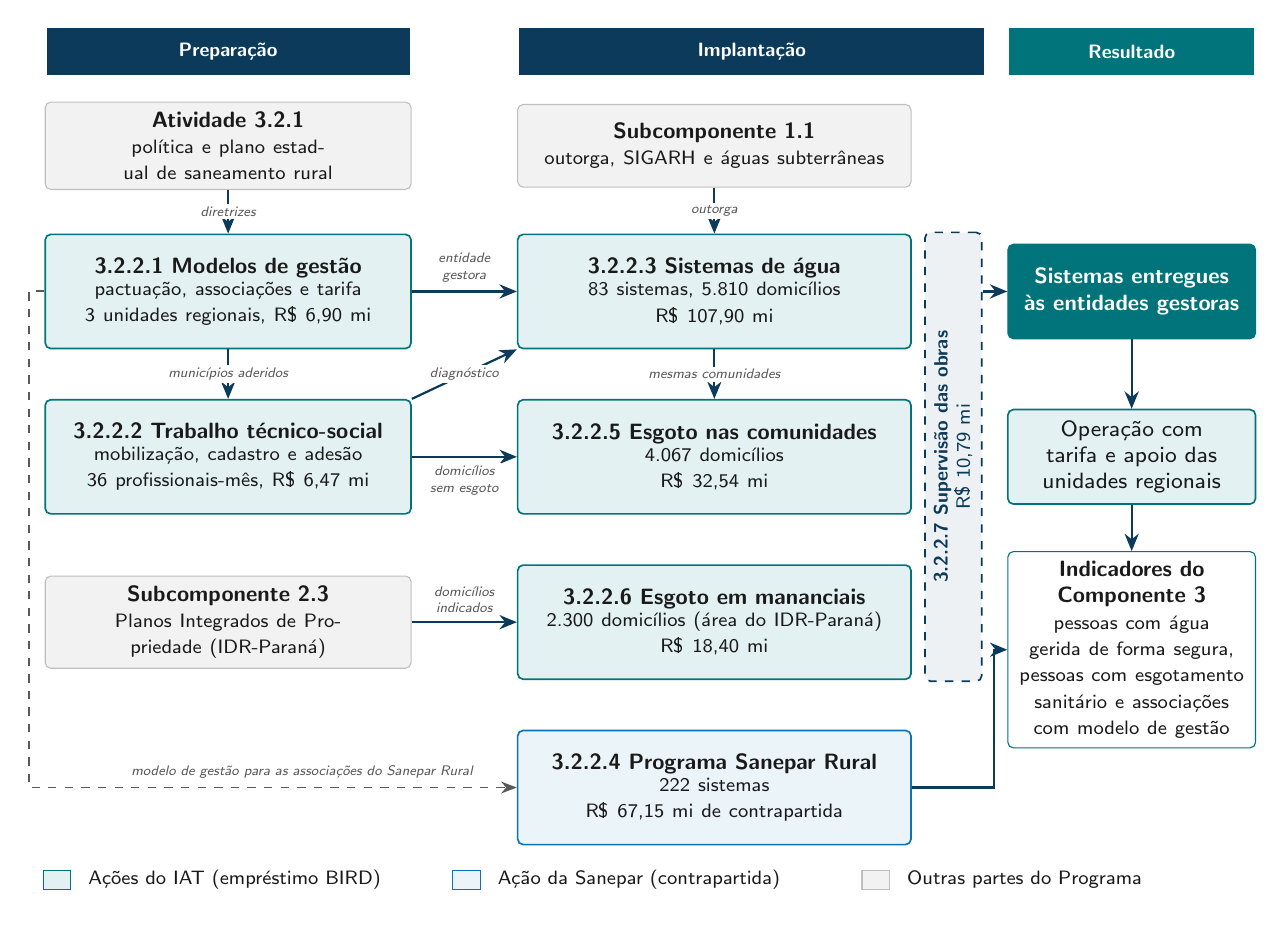
\begin{tikzpicture}[
  acao/.style={etapa=4.75cm, minimum height=1.45cm},
  acao1/.style={etapa=4.4cm, minimum height=1.45cm},
  sane/.style={draw=cBlue, fill=cBlueBg, rounded corners=2pt, align=center, inner sep=3.5pt,
    minimum height=1.45cm, text width=4.75cm, line width=0.6pt},
  ext/.style={externo=4.75cm, minimum height=1.05cm},
  ext1/.style={externo=4.4cm, minimum height=1.05cm},
  lig/.style={font=\tiny\itshape, text=cGrayText, fill=white, inner sep=1pt, align=center}
]
  \node[cab=4.4cm] (h1) at (2.45,0) {Preparação};
  \node[cab=5.7cm] (h2) at (9.1,0) {Implantação};
  \node[cab=2.9cm, fill=cTeal] (h3) at (13.925,0) {Resultado};

  \node[ext1] (x1) at (2.45,-1.2) {\textbf{Atividade 3.2.1}\\ {\scriptsize política e plano estadual de saneamento rural}};
  \node[ext] (x3) at (8.625,-1.2) {\textbf{Subcomponente 1.1}\\ {\scriptsize outorga, SIGARH e águas subterrâneas}};

  \node[acao1] (a1) at (2.45,-3.05) {\textbf{3.2.2.1 Modelos de gestão}\\
    {\scriptsize pactuação, associações e tarifa\\ 3 unidades regionais, R\$ 6,90 mi}};
  \node[acao1] (a2) at (2.45,-5.15) {\textbf{3.2.2.2 Trabalho técnico-social}\\
    {\scriptsize mobilização, cadastro e adesão\\ 36 profissionais-mês, R\$ 6,47 mi}};
  \node[ext1] (x2) at (2.45,-7.25) {\textbf{Subcomponente 2.3}\\ {\scriptsize Planos Integrados de Propriedade (IDR-Paraná)}};

  \node[acao] (b1) at (8.625,-3.05) {\textbf{3.2.2.3 Sistemas de água}\\
    {\scriptsize 83 sistemas, 5.810 domicílios\\ R\$ 107,90 mi}};
  \node[acao] (b2) at (8.625,-5.15) {\textbf{3.2.2.5 Esgoto nas comunidades}\\
    {\scriptsize 4.067 domicílios\\ R\$ 32,54 mi}};
  \node[acao] (b3) at (8.625,-7.25) {\textbf{3.2.2.6 Esgoto em mananciais}\\
    {\scriptsize 2.300 domicílios (área do IDR-Paraná)\\ R\$ 18,40 mi}};
  \node[sane] (b4) at (8.625,-9.35) {\textbf{3.2.2.4 Programa Sanepar Rural}\\
    {\scriptsize 222 sistemas\\ R\$ 67,15 mi de contrapartida}};

  \node[draw=cNavy, fill=cNavy!7, dashed, rounded corners=2pt, line width=0.6pt,
        fit={(11.3,-2.3) (12.02,-8.0)}, inner sep=0pt] (band) {};
  \node[rotate=90, font=\scriptsize, text=cNavy, align=center] at (band.center)
    {\textbf{3.2.2.7 Supervisão das obras}\\ R\$ 10,79 mi};

  \node[marcoteal=2.9cm, minimum height=1.2cm] (c1) at (13.925,-3.05) {Sistemas entregues às entidades gestoras};
  \node[etapa=2.9cm, minimum height=1.2cm] (c2) at (13.925,-5.15) {Operação com tarifa e apoio das unidades regionais};
  \node[draw=cTeal, fill=white, rounded corners=2pt, align=center, text width=2.9cm,
        inner sep=3.5pt, minimum height=1.3cm] (c3) at (13.925,-7.6)
        {\textbf{Indicadores do Componente 3}\\ {\scriptsize pessoas com água gerida de forma segura, pessoas com esgotamento sanitário e associações com modelo de gestão}};

  \draw[seta] (x1) -- (a1) node[lig, midway] {diretrizes};
  \draw[seta] (x3) -- (b1) node[lig, midway] {outorga};
  \draw[seta] (a1) -- (a2) node[lig, midway] {municípios aderidos};
  \draw[seta] (a1) -- (b1) node[lig, midway, above=2pt] {entidade\\ gestora};
  \draw[seta] (a2.north east) -- (b1.south west) node[lig, pos=0.5] {diagnóstico};
  \draw[seta] (a2) -- (b2) node[lig, midway, below=2pt] {domicílios\\ sem esgoto};
  \draw[seta] (b1) -- (b2) node[lig, midway] {mesmas comunidades};
  \draw[seta] (x2) -- (b3) node[lig, midway, above=2pt] {domicílios\\ indicados};
  \draw[seta] (band.east |- c1) -- (c1.west);
  \draw[seta] (c1) -- (c2);
  \draw[seta] (c2) -- (c3);
  \draw[seta] (b4.east) -- (12.18,-9.35) |- (c3.west);
  \draw[setatracejada] (a1.west) -- ++(-0.2,0) |- (b4.west)
    node[lig, pos=0.78, above=2pt] {modelo de gestão para as associações do Sanepar Rural};

  \begin{scope}[shift={(0.1,-10.65)}]
    \fill[cTealBg, draw=cTeal] (0,0) rectangle (0.35,0.25);
    \node[anchor=west, font=\scriptsize] at (0.45,0.125) {Ações do IAT (empréstimo BIRD)};
    \fill[cBlueBg, draw=cBlue] (5.2,0) rectangle (5.55,0.25);
    \node[anchor=west, font=\scriptsize] at (5.65,0.125) {Ação da Sanepar (contrapartida)};
    \fill[cGrayBg, draw=cGrayLine] (10.4,0) rectangle (10.75,0.25);
    \node[anchor=west, font=\scriptsize] at (10.85,0.125) {Outras partes do Programa};
  \end{scope}
\end{tikzpicture}

\end{document}
